% Kelompok : 5
% Kelas : D4 TI 1A
% Anggota : 
% 1. Harun Ar - Rasyid 	1174027
% 2. Choirul Anam 		1174004
% 3. M.Tomy N.M.		1174031
% 4. Izza				1174013
% 5.Putra				


Artikel ini mengenai segmentation

  \begin{figure}[ht]
  \centerline{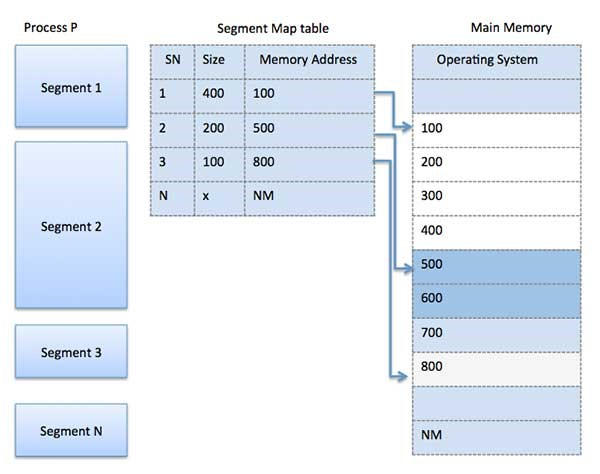
\includegraphics[width=1\textwidth]{..figures/segmentation.jpg}}
  \caption{Contoh segmentation}
  \label{segmentation}
  \end{figure}

\section{Pengertian Segmentation}
ini adalah contoh segmentation \ref{segmentation}
Segmentasi adalah teknik manajemen memori di mana setiap pekerjaan dibagi menjadi beberapa segmen dengan ukuran yang berbeda, satu untuk setiap modul yang berisi potongan-potongan yang melakukan fungsi terkait. Setiap segmen sebenarnya merupakan ruang alamat logis yang berbeda dari program. Ketika sebuah proses akan dieksekusi, segmentasinya yang sesuai akan dimuat ke dalam memori yang tidak bersebelahan meskipun setiap segmen dimuat ke dalam blok memori yang berdekatan dengan segmen lainnya.
Segmentasi manajemen memori bekerja sangat mirip dengan paging tetapi segmen di sini adalah variabel-panjang di mana seperti dalam halaman paging adalah ukuran tetap.
Segmen program berisi fungsi utama program, fungsi utilitas, struktur data, dan sebagainya. Sistem operasi memelihara tabel peta segmen untuk setiap proses dan daftar blok memori bebas bersama dengan nomor segmen, ukurannya dan lokasi memori yang sesuai dalam memori utama. Untuk setiap segmen, tabel menyimpan alamat awal segmen dan panjang segmen.
Segmen biasanya cocok atau sesuai dengan divisi alami dari suatu program seperti rutinitas individu atau tabel data sehingga segmentasi umumnya lebih terlihat oleh programmer daripada paging saja.  Segmen yang berbeda dapat dibuat untuk modul program yang berbeda, atau untuk kelas yang berbeda dari penggunaan memori seperti kode dan segmen data. 
\subsection{Implementasi perangkat keras}
Dalam sistem yang menggunakan segmentasi, alamat memori komputer terdiri dari id segmen dan offset dalam segmen tersebut. Sebuah unit manajemen memori perangkat keras (MMU) bertanggung jawab untuk menerjemahkan segmen dan mengimbangi ke alamat fisik, dan untuk melakukan pemeriksaan untuk memastikan terjemahan dapat dilakukan dan referensi ke segmen dan offset tersebut diizinkan.
Setiap segmen memiliki panjang dan serangkaian izin (misalnya, baca, tulis, jalankan) yang terkait dengannya. Suatu proses hanya diperbolehkan untuk membuat referensi ke dalam segmen jika jenis referensi diizinkan oleh izin, dan jika offset dalam segmen berada dalam rentang yang ditentukan oleh panjang segmen. Jika tidak, pengecualian perangkat keras seperti kesalahan segmentasi dinaikkan.
Segmen juga dapat digunakan untuk mengimplementasikan memori virtual. Dalam hal ini setiap segmen memiliki bendera terkait yang menunjukkan apakah ia ada dalam memori utama atau tidak. Jika segmen diakses yang tidak ada dalam memori utama, pengecualian dibangkitkan, dan sistem operasi akan membaca segmen ke dalam memori dari penyimpanan sekunder.
Dan juga tujuan dari yang biasa kita sebut dengan tahapan implementasi ini biasanya digunakan untuk memastikan bahwa software berjalan dengan efektif sesuai dengan apa yang diinginkan dalam membantu dalam penyelesaian dan pematangan dalam kosep pengembangan sistem jaringan menjadi lebih maju dan tentunya lebih efektif. ada 2 tipe segmentasi dalam implementasi perangkat yaitu segmentasi tanpa paging dan dengan paging
\subsubsection {Segmentasi Tanpa Paging}
Terkait dengan setiap segmen adalah informasi yang menunjukkan di mana segmen berada dalam memori — basis segmen. Ketika sebuah program referensi lokasi memori offset ditambahkan ke basis segmen untuk menghasilkan alamat memori fisik.